%! TEX program = luatex
%% ****** Start of file aiptemplate.tex ****** %
%%
%%   This file is part of the files in the distribution of AIP substyles for REVTeX4.
%%   Version 4.1 of 9 October 2009.
%%
%
% This is a template for producing documents for use with 
% the REVTEX 4.1 document class and the AIP substyles.
% 
% Copy this file to another name and then work on that file.
% That way, you always have this original template file to use.
% chktex-file 36
\documentclass[aps,prl,preprint,superscriptaddress]{revtex4-1} % chktex 8
%\documentclass[aip,reprint]{revtex4-1}
\usepackage{amsmath}
\usepackage{graphicx}
\usepackage{siunitx}
%\usepackage[english]{babel}
%\usepackage{upgreek}
%\usepackage[math-style=ISO]{unicode-math}
%\usepackage[upright]{fourier}
%\usepackage{newtxmath}
\usepackage{xcolor}
\bibliographystyle{plain}
\raggedbottom%
\def\nm{\,\si{\nano\meter}}% 
\draft% marks overfull lines with a black rule on the right
\begin{document}

% Use the \preprint command to place your local institutional report number 
% on the title page in preprint mode.
% Multiple \preprint commands are allowed.
%\preprint{}

\title{Magnetic-field Assisted Assembly of Colloidal Ellipsoids}

% repeat the \author .. \affiliation  etc. as needed
% \email, \thanks, \homepage, \altaffiliation all apply to the current author.
% Explanatory text should go in the []'s, 
% actual e-mail address or url should go in the {}'s for \email and \homepage.
% Please use the appropriate macro for the type of information

% \affiliation command applies to all authors since the last \affiliation command. 
% The \affiliation command should follow the other information.

%\author{}

\author{Antara Pal}
\email{antara.pal@fkem1.lu.se}
\affiliation{Division of Physical Chemistry, Department of Chemistry, Lund University, Lund, Sweden}
\author{Thiago H.Ito}
\affiliation{Division of Physical Chemistry, Department of Chemistry, Lund University, Lund, Sweden}
\author{Md. Arif Kamal}
\affiliation{Centre Interdisciplinaire de Nanoscience de Marseille (CINaM), CNRS, Aix Marseille University, Marseille, France}
\altaffiliation[Current Address: ]{Division of Physical Chemistry, Department of Chemistry, Lund University, Lund, Sweden}
\author{Andrei V. Petukhov}
\affiliation{Van't Hoff Laboratory for Physical and Colloid Chemistry, Utrecht University, The Netherlands}
\author{Peter Schurtenberger}
\email{peter.schurtenberger@fkem1.lu.se}
\affiliation{Division of Physical Chemistry, Department of Chemistry, Lund University, Lund, Sweden}

% Collaboration name, if desired (requires use of superscriptaddress option in \documentclass). 
% \noaffiliation is required (may also be used with the \author command).
%\collaboration{}
%\noaffiliation

\date{\today}

\begin{abstract}
%-----------------------------------------------------
Anisotropic colloids exhibit a rather complex and rich phase behavior in comparison to their isotropic analogues, which renders them as interesting model systems in various areas of condensed matter physics and materials science. Herein we present our investigations on the influence of an external magnetic field on the self-assembly of hematite-silica core-shell ellipsoidal colloids. In the presence of an external field, prolate particles at concentrations usually orient with their long axes along the field direction. However, our study has brought to light a rather counterintuitive but interesting phenomenon where \emph{prolate} anisotropic colloids self-assemble into \emph{oblate} liquid crystalline (LC) phases. This \emph{unusual} self-assembly behaviour can be attributed to an inherent peculiarity in the magnetic property of hematite, due to which, the particles align with their short axes along the field direction. Detailed characterization of the concentration dependent self-assembly process using particles with two different but relatively small aspect ratios (AR) reveal that self-assembly is sensitive to the particle AR\@. For particles with smaller AR, an increase in concentration results in the formation of a sequence of oblate LC phases: \emph{para-nematic}, \emph{nematic}, \emph{smectic} and an \emph{oriented glass}. Remarkably, the occurrence of Smectic phase in colloidal ellipsoidal systems has neither been predicted by simulations nor previously reported experimentally. Our study unequivocally demonstrates the power of combining anisotropic building blocks and external fields as a route towards field-directed self-assembly of novel structures with externally tunable properties. 
%-----------------------------------------------------
\end{abstract}

\pacs{}% insert suggested PACS numbers in braces on next line

\maketitle {}%\maketitle must follow title, authors, abstract and \pacs

% Body of paper goes here. Use proper sectioning commands. 
% References should be done using the \cite, \ref, and \label commands
\section{Introduction}
%\label{}
%-----------------------------------------------------------------------------------------------------------------------------------
Over the past couple of decades the focus of colloid science has gradually witnessed an evermore shift towards understanding the behavior of anisotropic particles; particles having anisotropy either in their shape or interaction potential or both. Anisotropic colloids exhibit a rather complex and rich phase behavior in comparison to their isotropic analogues, which makes them particularly interesting model systems in various areas of condensed matter physics and materials science. The prospect of tuning their self-organization by modifying the anisotropy in their shape in conjunction with the possibility of introducing an anisotropy in the interaction potential using external fields have ushered in a new paradigm towards the understanding, design and control of novel self-assembled materials. \par
%-----------------------------------------------------------------------------------------------------------------------------------
Depending upon the particle shape and the interaction potential, suspensions of aniso\-tropic colloids manifest different
self-assembled structures encompassing the \emph{isotropic}, 
\emph{nematic}~\cite{pizzey2004suspensions, van1998formation, purdy2005nematic, buining1993isotropic, fraden1989isotropic, lemaire2002outstanding, lemaire2004physical, vroege2014biaxial, van2010uniaxial, rossi2010cholesteric, li2016colloidal,dogic2016filamentous}, 
\emph{smectic}~\cite{davidson2018isotropic, vroege2006smectic, kuijk2012phase} and \emph{columnar} phases~\cite{van2000liquid, brown1999phase, wijnhoven2005sedimentation, van2004liquid, van2005evidence}. 
One of the most important feature that distinguishes these phases from one another is the presence (or absence) of orientational and positional order. In the isotropic phase the particles possess neither 
orientational nor positional order, where as in the nematic phase there exists a long-range orientational order but there is an absence of long-range positional order. 
Smectic and the crystal phases are generally characterized by the presence of both long-range orientational as well as positional order. \par
%-----------------------------------------------------------------------------------------------------------------------------------
The use of external electromagnetic fields to manipulate the orientational interactions of anisotropic particles and drive their self-assembly has been in the spotlight for the last couple of years (ref.~\cite{op2013phase, Schurtenberger2016, ganesan2017high, shah2015actuation} and references therein). The fast and reversible nature of the field-induced dipole-dipole interaction between the particles, as is the case in these systems, makes this bottom-up approach extremely versatile. In view of the ease in manipulating the interaction potential of the magnetic particles through external field, we have in the present study focused our attention towards investigating the field-directed self-assembly of ellipsoidal particles with a magnetic core.\par
%-----------------------------------------------------------------------------------------------------------------------------------
Over the past decade a significant amount of work has been done towards elucidating the theoretical phase diagrams for ellipsoidal particles. These studies predict the existence of isotropic, nematic and SM2 crystalline phases as a function of concentration and axial ratio~\cite{radu2009solid, odriozola2012revisiting, pfleiderer2008crystal}. It is interesting to note that so far there are neither any predictions nor any experimental reports for the existence of a smectic phase in case of ellipsoidal particles. This is stark contrast to the situation encountered for example of particles with cylindrical or spherocylindrical shapes~\cite{Bolhuis1997, lekkerkerker2013liquid}. In this article we have not only revisited these theoretical predictions for ellipsoidal particles, but have in addition used an external field to investigate the effect of a partial reduction in the rotational degrees of freedom of the ellipsoids.\par
%%%----------------------------------------------------------------------------------------------
In the case of anisotropic particles, presence of an external magnetic field results in an alignment of the magnetic moment of the individual particles along the field direction, thereby restricting rotational motion of the particles accordingly. For prolate particles the induced dipolar moments are in general along their long axis. However, this is not the case for the prolate particles consisting of a magnetic core that is made up of hematite ($\alpha$-Fe$_2$O$_3$) spindles. In this scenario, the particles align with their short axis parallel to the field direction. Explanation of this rather uncanny behaviour rests on the fact that in case of hematite the easy axis of magnetization resides within the basal plane of the hematite and is oriented perpendicular to the spindle axis~\cite{reufer2011magnetization}. Consequently, the direction of the induced magnetic moments is perpendicular to the long axes. Although at sufficiently large field strengths the particles align with their short axis parallel to the magnetic field, they can however still individually rotate around their magnetic moments provided the volume fraction is low enough and interparticle interactions are negligible~\cite{reufer2010morphology}. \par
%---------------------------------------------------------------------
In the present article, we have exploited aforementioned property of hematite to tune the self-assembly of colloidal ellipsoids for two different aspect ratios of $\rho = 2.82$ and $\rho = 3.69$ at different concentrations. Using gravity to create a sedimentation profile (or concentration gradient) in a dispersion of silica coated hematite ellipsoids allows us to efficiently sample a large range of the phase space within a single sample. We report that for the ellipsoidal particles with the smaller aspect ratio ($\rho=2.82$) four different self-assembled structures exist: \emph{para-nematic}, \emph{nematic}, \emph{smectic} and \emph{oriented glass}, respectively. A quantitative analysis of the SAXS patterns clearly reveals that it is possible to create oblate self-assembled phases with prolate particles through the application of an external field. Astonishingly, our data unambiguously demonstrates the existence of a smectic phase in a colloidal ellipsoidal system, which has been neither predicted by simulations nor previously found experimentally. In the smectic phase, the SAXS pattern exhibits a curious peak shape that resembles a \textit{paper-clip} with highly anisotropic tails along the direction of the smectic periodicity. The presence of this unusual peak structure is rationalized by the modulation of the intensity in the form of a spherocylinder due to the correlation between the particles along different directions together with a layer undulation. In contrast, ellipsoids with higher aspect ratio, $\rho=3.69$ were found to self-assemble in only two different phases --- \emph{para-nematic} and \emph{nematic}, demonstrating the importance of shape anisotropy in field-directed self-assembly.
%---------------------------------------------------------------------
\begin{figure}[!h]
\centering{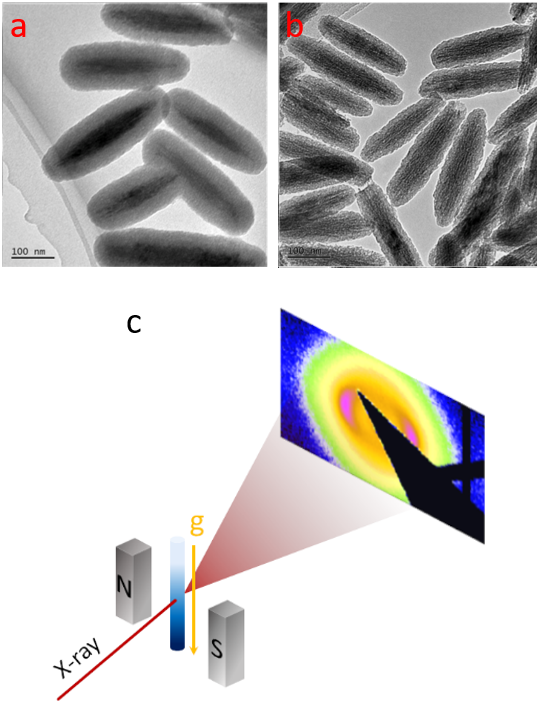
\includegraphics[width=0.5\linewidth]{TEM_2.png}}
\caption{TEM images for ellipsoidal colloids for aspect ratios (a) $\rho_1=2.82$ and (b) $\rho_2=3.69$. (c) Experimental set-up for SAXS measurement.}\label{TEM}
\end{figure}
%----------------------------------------------------------------------------------------------------------------
\section{Results and discussion}
%----------------------------------------------------------------------------------------------------------------
\subsection{Sample $E1$ with aspect ratio $\rho_1 = 2.82$}
%----------------------------------------------------------------------------------------------------------------
\begin{figure*}[t]
\centering{\includegraphics[width=0.95\textwidth]{Figure_Zscan_06.png}}
\caption{Typical 2D diffraction patterns for (a) para-nematic, (b) nematic, (c) smectic and (d) oriented glass phases at different heights of the sedimented sample for $\rho=2.82$. The variation of the scattered intensity as a function of scattering vector, $q$, for the aforementioned self-assembled phases along the direction of the external field (e) and perpendicular to it (f). (g) The variation of the nearest neighbor distance, $d$, and the FWHM of the nearest neighbor peaks as a function of height, $Z$ from the bottom of the capillary have been represented by the blue circles and the red squares respectively. The bottom panel represents schematic of the aforementioned self-assembled phases.}\label{z_scan}
\end{figure*} 
%----------------------------------------------------------------------------------------------------------------
The ellipsoidal system studied here exhibits a rich phase behavior involving para-nematic (pN)\footnote{pN phase has been described before as polarized fluid in ref.~\cite{martchenko2016anisotropic}}, nematic (N), smectic (S) and oriented glass (OG) phases. At the top of the sedimentation profile the concentration is relatively low, resulting in weak inter-particle correlations. As a result, the field-induced torque is mostly exerted onto single particles, resulting in an alignment that leads to the formation of a para-nematic phase (Fig.\ref{z_scan}(a)). A nematic phase followed by a smectic one is observed as one moves lower down in the capillary (Fig.~\ref{z_scan}(b), (c)). At the bottom of the sediment, due to very high concentration, the particles form a kinetically arrested glass phase. In the presence of an external field, the particles tend to align with their short axes parallel to the field direction. As a result, the glass phase develops an anisotropy (Fig.\ref{z_scan}(d)). The nematic phase found for colloidal rods, which align their long axis, is often referred to as a \emph{prolate nematic}, N$_+$, while plate-like colloids exhibit an \emph{oblate nematic}, N$_-$, where the short particle axes are aligned. It is interesting to note that despite the prolate shape of our ellipsoidal particles their orientational behaviour in the presence of the external field closely follows that of oblate particles. This behaviour can be rationalized when one considers the fact that the ellipsoids consist of a hematite core. As a result, their magnetic moments lie along the short axes of the particles. Under the influence of an external magnetic field these particles self assemble with their short axes parallel to the field direction, thereby resembling oblate particles rather than rods. One can therefore refer to the field induced nematic, smectic and para-nematic phases as N$_-$, S$_-$ and pN$_-$ respectively which is in strong contrast to the phases observed for colloidal rods~\cite{kuijk2011synthesis}. \par
%----------------------------------------------------------------------------------------------------------------
Fig.\ref{z_scan}(e) and (f) represent one-dimensional intensity profiles for different phases along and perpendicular to the direction of the field, respectively. At the very top of the sediment, in the pN phase, one can observe only the form factor, which is highly anisotropic; extending to larger $q$ along the field direction and decaying much faster in a direction perpendicular to the field direction (Fig.\ref{z_scan}(e)(f)(red)). This indicates that the particles are aligned with their short axes parallel to the field direction. At sufficiently high concentrations, positional correlations start to play an important role for the scattering in the direction parallel to the magnetic field. As a result, the static structure factor dominates the intensity profile, and we observe the appearance of additional well-developed maxima. The presence of very sharp smectic reflections up to fourth order along the direction of the field indicates a highly ordered structure (Fig.\ref{z_scan}(e)(cyan)). These strong positional and orientational correlations disappear again at the highest concentrations in the OG phase, where only a clear structure factor peak related to side-by-side correlations of the particles is observed parallel to the field direction(Fig.\ref{z_scan}(e)(blue)). In contrast, the scattering features are much less clearly developed in a direction normal to the field direction, and we only observe weak correlation peaks originating from the tip-to-tip configurations, i.e., with a separation distance equal to the particle length, for the nematic, smectic and oriented glass phases (Fig.\ref{z_scan}(f)). \par
%----------------------------------------------------------------------------------------------------------------
Along the direction of the field, the nearest neighbor distance $d$ $(=2\pi/q_{max})$ increases as a function of $Z$ (Fig.\ref{z_scan}(g)), reflecting the decrease in concentration with increasing sample height. The full-width at half-maximum (FWHM) of the diffraction peak, which represents the inverse of the positional correlations, also changes as a function of $Z$ (Fig.\ref{z_scan}(g)). For the oriented glass and the nematic phase, the FWHM is quite large, indicating the presence of liquid-like positional order. In case of the smectic phase, however, there is a sharp decrease in FWHM, demonstrating the existence of a one-dimensional crystalline order.\par   % chktex 35
%----------------------------------------------------------------------------------------------------------------
\subsubsection{Characterization of the Nematic Phase}
%----------------------------------------------------------------------------------------------------------------
\begin{figure}[ht]
\centering{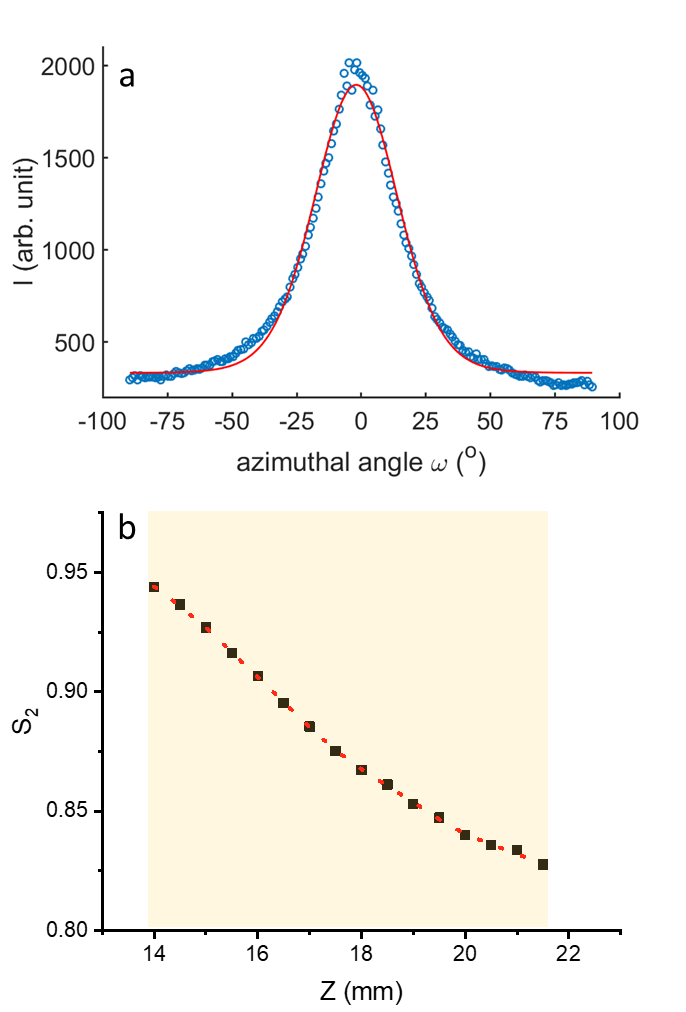
\includegraphics[width=0.5\linewidth]{order_param_5.png}}
\caption{(a) The blue circles represent the azimuthal intensity profile along the red dashed line shown in Fig.\ref{z_scan}(b) and the corresponding fit using eq.\ref{eq2:}(red line). (b) The variation of the orientational order parameter $S_2$ as a function of $Z$ in the nematic phase. The red dashed line is a guide to the eye but not a fit.}\label{order_param}
\end{figure} 
%----------------------------------------------------------------------------------------------------------------
The nematic phase is characterized by short-range positional order but long-range orientational order, which can be represented with the help of an orientational order parameter, $S_2$. Following Purdy \emph{et.~al.}~\cite{purdy2003measuring, kleshchanok2010structures}, the azimuthal intensity distribution (along the red dashed line in Fig.~\ref{z_scan}(b)) can be fitted with,
%----------------------------------------------------------------------------------------------------------------
\begin{equation}
\label{eq2:}
%\begin{split}
I= baseline +  I_0 f(\omega)
%\end{split}
\end{equation} 
%----------------------------------------------------------------------------------------------------------------
\noindent where $I_0$ is the normalizing factor, $\omega$ is the azimuthal angle and $f(\omega)$ is the orientational distribution function,
%----------------------------------------------------------------------------------------------------------------
\begin{equation}
\label{eq3:}
%\begin{split}
f(\omega)=\exp(-AP(\omega))
%\end{split}
\end{equation} 
%----------------------------------------------------------------------------------------------------------------
%\noindent where $A$ is the width of the Legendre polynomial,
\noindent where the parameter $A$ determines the width of the distribution function and $P(\omega)$ is the Legendre polynomial
%----------------------------------------------------------------------------------------------------------------
\begin{equation}
\label{eq4:}
%\begin{split}
P(\omega)=\frac{1}{2}(3\cos^2(\omega-\omega_0)-1)
%\end{split}
\end{equation} 
%----------------------------------------------------------------------------------------------------------------
\noindent $\omega_0$ being the tilt angle. The orientational order parameter, $S_2$, can now be obtained by,
%----------------------------------------------------------------------------------------------------------------
\begin{equation}
\label{eq5:}
%\begin{split}
S_2= \frac{\int f(\omega)P(\omega)\sin(\omega)d\omega}{\int f(\omega)\sin(\omega)d\omega}
%\end{split}
\end{equation}
%----------------------------------------------------------------------------------------------------------------
\noindent Fig.\ref{order_param}(a) shows a representative fit of the experimental data with the Purdy model, while Fig.\ref{order_param}(b) represents the variation of $S_2$ as a function of $Z$. The analysis reveals that one of the short axes of the ellipsoids are very well aligned throughout the nematic phase, resulting in an order parameter $>$ 0.8. An interesting observation is that the order parameter is larger at the bottom part, indicating that the sample is more ordered, which is expected due to the sedimentation induced concentration gradient.\par
%------------------------------------------------------------------------------------------------------------------
\subsubsection{Characterization of the Smectic Phase}
%------------------------------------------------------------------------------------------------------------------
\begin{figure}[ht]
\centering{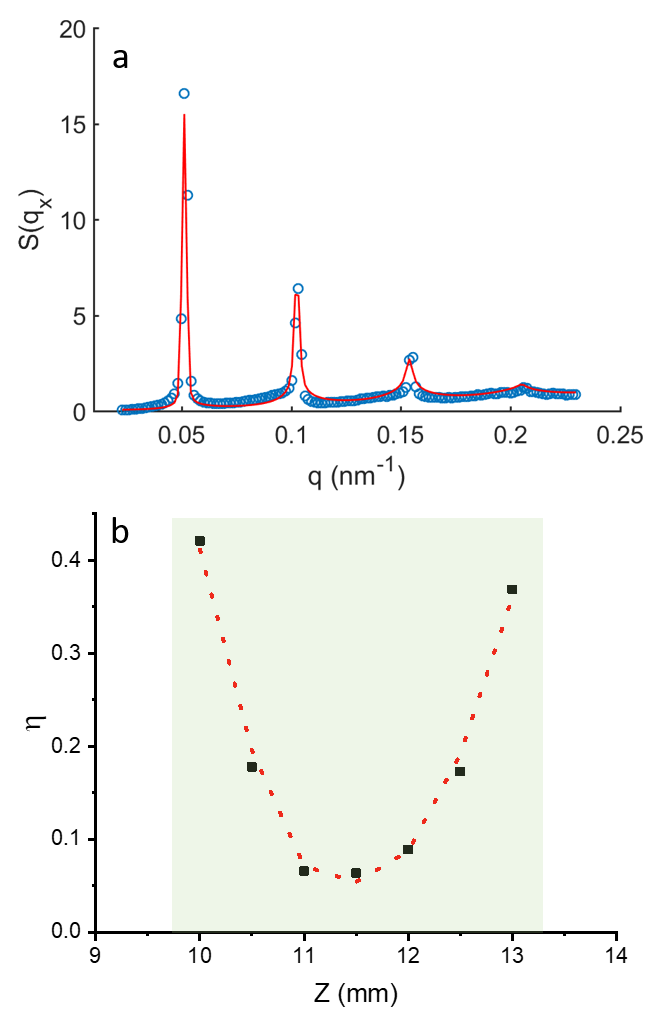
\includegraphics[width=0.5\linewidth]{callie_6.png}}
\caption{(a) Experimental structure factor along the field direction shown by red dashed line in Fig.\ref{z_scan}(c) (blue circles) along with the fit (red line) using the Nallet model described by eq.\ref{eq1:} for the smectic phase at a height $Z=11.5mm$ from the bottom of the capillary. (b) Variation of the Calli\`{e} parameter as a function of $Z$ for the smectic phase. The red dashed line is a guide to the eye but not a fit.}\label{callie}
\end{figure}
%----------------------------------------------------------------
\begin{figure*}[ht]
\centering{\includegraphics[width=0.95\textwidth]{Figure_Fspace_smectic_5.png}}
\caption{Schematic representation of (a) the alignment of the ellipsoids in an external field in real space. Since they align with their short axes being parallel to the field direction, they get confined in 2D planes (shown in gray) perpendicular to the direction of the field, (b) the corresponding 3D Fourier space representation of the structure factor variation in the form of a cylinder. (c) Once these layers start to get correlated, sharp Bragg spots start to appear on the axis of this cylindrical structure factor. The orange plane represents the detector plane. (d) Expected diffraction pattern on the detector plane. The sharp Bragg spots become arcs because of polycrystallinity.}\label{Fspace_smectic}
\end{figure*} 
%----------------------------------------------------------------------------------------------------------------
The smectic phase is most commonly observed for amphiphilic systems where amphiphiles self-assemble in the form of bilayers, which then stack together to form a lamellar phase. We have characterized the smectic phase by borrowing the knowledge from the lamellar phase. The radially integrated structure factor $S(q_x)$ of the smectic phase can be obtained by dividing the recorded intensity, $I$, by the form factor ($\propto q_x^{-2}$). The resolution ($\Delta q$) limited $S(q_x)$ can now be described by the Nallet model~\cite{nallet1993modelling}, 
%----------------------------------------------------------------------------------------------------------------
\begin{equation}
\label{eq1:}
\begin{split}
S(q_x) = &1+2\sum_{n=1}^{N-1} (1-\frac{n}{N}) +\cos(\frac{q_x d n}{1+2\Delta q^2 d^2 \alpha(n)})\\
&\times\exp(-\frac{2q_x^2 d^2\alpha(n)+\Delta q^2 d^2 n^2}{2(1+2\Delta q^2 d^2 \alpha(n))})\frac{1}{\sqrt{1+2\Delta q^2 d^2 \alpha (n)}}
%\rho_{part}  = \frac{1}{{a_{part}b_{part^2}}} &\left[a_{core}b_{core}^2\{\rho_{sil}\phi_{pores}^{core}+\rho_{hem}(1-\phi_{pores}^{core})\} \right.\\
%& \left.+(a_{part}b_{part}^2-a_{core}b_{core}^2)\{\rho_{wtr}\phi_{pores}^{shell}+\rho_{hem}(1-\phi_{pores}^{shell})\}\right]
\end{split}
\end{equation}
%----------------------------------------------------------------------------------------------------------------
\noindent with $\alpha(n)=\frac{\eta}{4\pi^2}(\ln \pi n + \gamma)$. Here, $\gamma$ is Euler's contant and $\eta$ is the Caill\'{e} parameter, which is a measure of the fluctuations in the system; $\eta=0$ means that there is no fluctuations, while in the presence of fluctuations $\eta$ increases and the higher order Bragg peaks are smoothed out. Fig.\ref{callie}(a) shows a representative fit of the experimental data with the Nallet model, while Fig.\ref{callie}(b) represents the variation of the estimated $\eta$ as a function of $Z$. One can observe that just above the glass phase, $\eta$ is quite high with a larger fluctuation in the system followed by a sharp decrease in $\eta$, representing a highly ordered smectic phase. However, fluctuations and hence $\eta$ again increases to a higher value close to the nematic phase.\par  
%---------------------------------------------------------------------------------------------------------------- % chktex 36
Further, a careful inspection of the diffraction pattern of the nematic and smectic phases reveals an unusual but interesting feature resembling \textit{paper-clip}(Fig.~\ref{z_scan}(b,c)) shapes. This peculiar shape of the diffraction pattern is more prominent in the smectic phase, where one can clearly notice diffuse scattering lines parallel to the direction of the smectic periodicity. In the absence of the external magnetic field, particles are randomly oriented in all possible directions (fig.~\ref{Fspace_smectic}(a)). As a result, in Fourier space the structure factor is expected to be modulated in the form of spherical shells as one can see in fig.~\ref{Fspace_smectic}(b), which in turn produces a circle on the detector plane (shown by the yellow planes in fig.~\ref{Fspace_smectic}(b,c)). Since a sphere is a three dimensionally symmetrical object, it does not matter at which angle the detector plane is passing through it to get a circular/isotropic diffraction pattern (fig.~\ref{Fspace_smectic}(d)). In presence of the external field, the particles tend to align with their short axes parallel to the field direction (fig.~\ref{Fspace_smectic}(e)). In turn, one of the rotational degrees of freedom freezes out, resulting in anisotropy in the Fourier space structure. Along the magnetic field the correlation distance is governed by the smaller particle dimension while in the orthogonal directions it is mainly dominated by their length. In the intermediate directions between these two, the gradual change of the typical correlation distance leads to this peculiar shape of the structure factor resembles like a spherocylinder (SC) as shown in fig.~\ref{Fspace_smectic}(f). % chktex 36
%In Fourier space, the structure factor becomes elongated along the direction corresponding to the short axes of the particles keeping the other two direction unchanged. As a result the structure factor is modulated in the form of a spherocylinder (SC) as shown in fig.~\ref{Fspace_smectic}(f).% chktex 12 
Now depending on the direction at which the detector plane intersects the Fourier space, one would expect to observe either a circle, ellipse or a two dimensional projection of a SC on the detector plane. For our experimental geometry, the detector plane passes parallel to the long axis of the three dimensional spherocylinder generated in the Fourier space and one would expect to see a structure factor modulated in the shape shown in fig.~\ref{Fspace_smectic}(g). This expected diffraction pattern matches exactly with what we observe in the experiment for the nematic phase (fig.~\ref{Fspace_smectic}(h)). With a further increase in concentration (i.e.~moving down in the capillary) the particles get confined in 2D planes with their long axes lying on the planes (Fig.~\ref{Fspace_smectic}(i)). These planes are normal to the field direction and within each plane particle ordering is \emph{liquid}-like. Beyond a certain concentration, correlation starts to build up between these planes resulting in a smectic phase. In an ideal smectic structure one would expect a sequence of sharp smectic reflections together with a broad intralayer scattering peak that is mostly broadened in a direction perpendicular to the layering direction. In contrast, what we observe is a paper-clip-like diffraction pattern. This peculiar shape suggests the presence of strong nematic-like fluctuations such as undulation of the smectic layers and correlations between the particles of different layers. While the correlations between the particles (that belong to different layers) along different directions lead to the horizontal diffused scattering line along the smectic periodicity, the layer undulations will lead to the appearance of the tails for higher-order Bragg peaks, which explains the multiple paper-clip-like features as highlighted in SI\@. The corresponding Fourier space structure is shown in fig.~\ref{Fspace_smectic}(j). The detector plane being parallel to the field direction and perpendicular to the x-ray beam (fig.~\ref{TEM}(c)) passes through the SC along its long axis to produce a diffraction pattern in the form of a paper-clip (fig.~\ref{Fspace_smectic}(k)) as one can observe in our experimental scattering pattern (fig.~\ref{Fspace_smectic}(l)).\par
%----------------------------------------------------------------------------------------------------------------
\begin{figure*}[t]
\centering{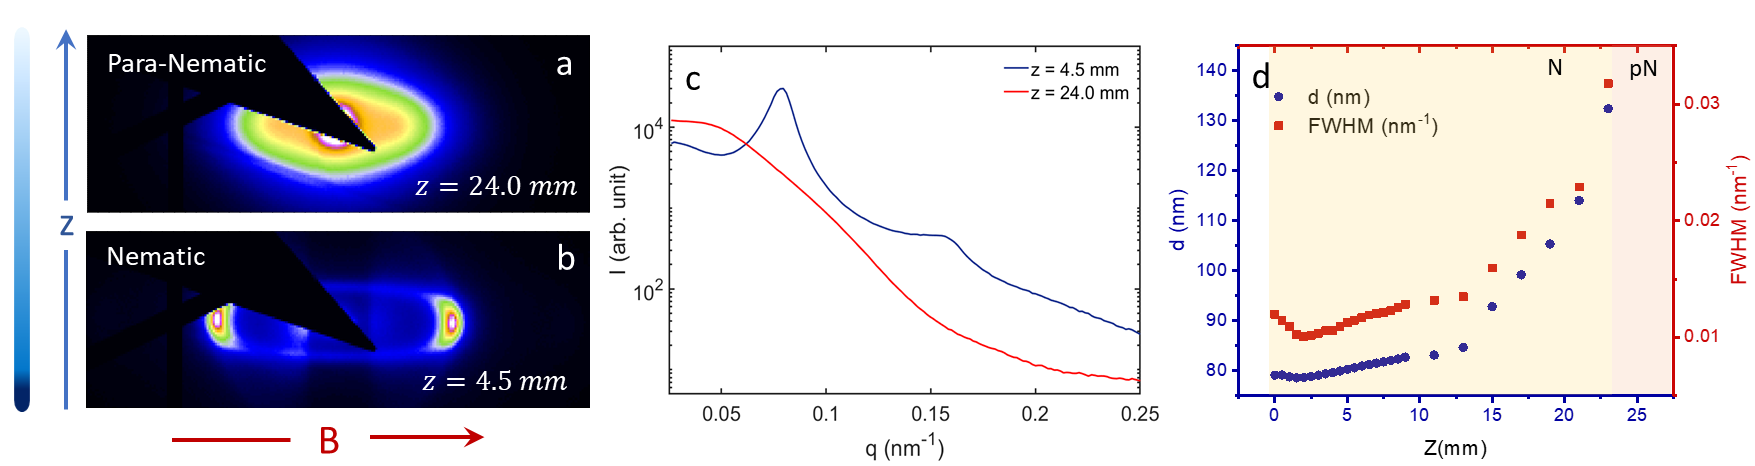
\includegraphics[width=0.95\textwidth]{z_scan_high_2.png}}
\caption{Typical 2D diffraction patterns for (a) para-nematic and (b) nematic phases at different heights of the sedimented sample for $\rho=3.69$. (c) The variation of the scattered intensity as a function of scattering vector, $q$, for the aforementioned self-assembled phases along the direction of the external field. (d) The variation of the nearest neighbor distance, $d$, and the FWHM of the nearest neighbor peaks as a function of height, $Z$ from the bottom of the capillary have been represented by the blue circles and the red squares respectively.}\label{z_scan_high}
\end{figure*}
%---------------------------------------------------------------------------------------------------------------
%A closer look at the diffraction pattern of the nematic phase reveals similar diffuse scattering features arising from the formation of cylindrical structure factor (Fig.\ref{z_scan}(c)).
%----------------------------------------------------------------------------------------------------------------
\subsection{Sample $E2$ with aspect ratio $\rho_1 = 3.69$}
%----------------------------------------------------------------------------------------------------------------
In contrast to the particles with lower aspect ratio, the ones with higher aspect ratio show only two different phases in the presence of the external field. At the top of the capillaries a para-nematic phase is observed, followed by a nematic phase at the bottom (Fig.~\ref{z_scan_high}(a),(b)). In this case, the diffuse scattering due to the formation of the spherocylindrical structure factor is much more prominent in the nematic phase (Fig.~\ref{z_scan_high}(b)) itself. Fig.~\ref{z_scan_high}(c) represents the one dimensional intensity profile for the nematic and para-nematic phase along the direction of the field. The nearest neighbor distance, \emph{d}, along the direction of the field increases with $Z$ in a similar way as that of sample $E1$ (Fig.\ref{z_scan_high}(d)). In contrast, FWHM is increasing monotonically since Sample $E2$ does not show any smectic phase (Fig.~\ref{z_scan_high}(d)). \par
%----------------------------------------------------------------------------------------------------------------
\subsection{Computer Simulations}
\begin{figure*}[ht]
\centering{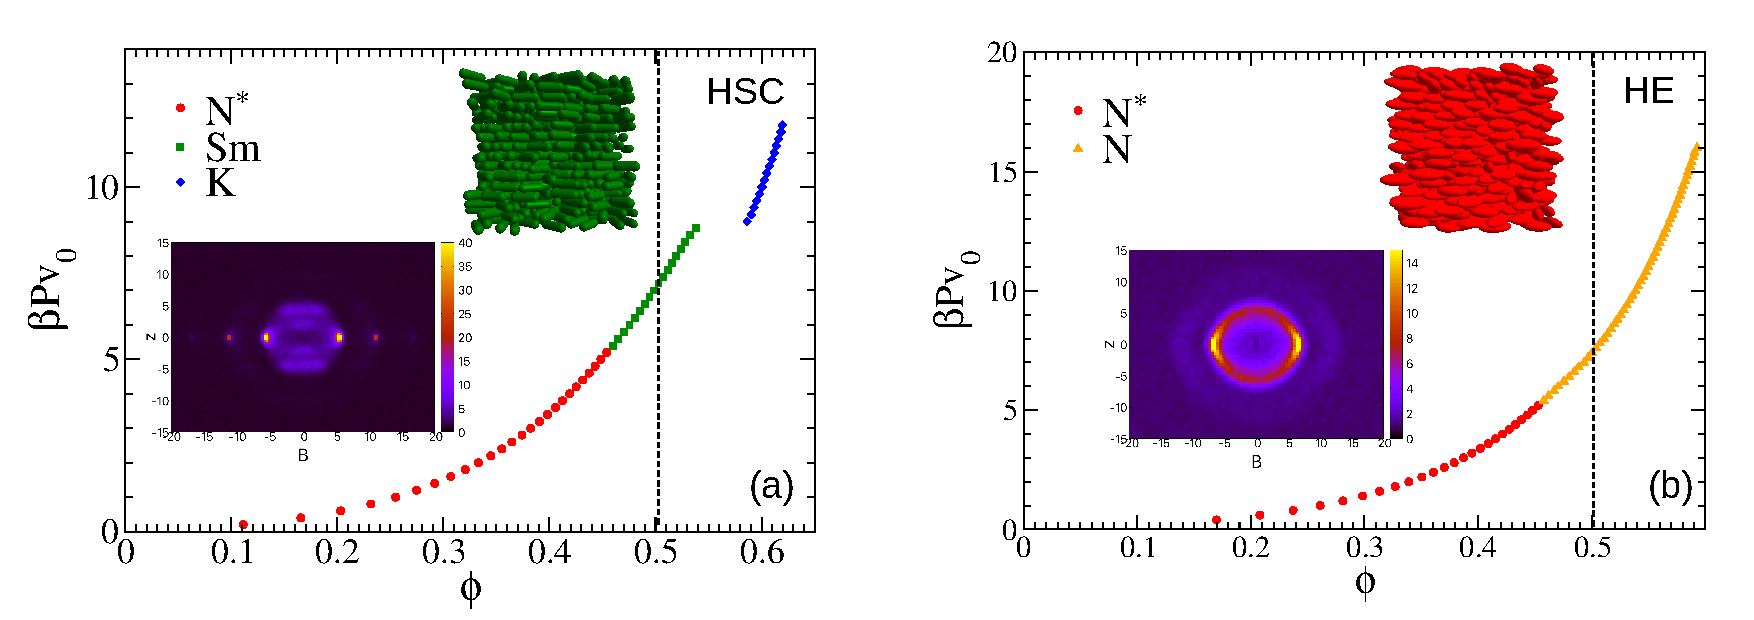
\includegraphics[width=0.95\textwidth]{mceos.pdf}}
\caption{Equation of states of (a) Hard Spherocylinders and (b) Hard Ellipsoids (right) from Monte Carlo simulations. 
  Insets show the static structure factors and snapshots for $\phi\approx 0.50$. 
Monte Carlo Simulations}\label{fig:sim}
\end{figure*}
Hematite-silica core-shell particles of aspect ratio $\rho_1$
have a rather peculiar hybrid shape, where their midsection is more cylinder-like, as the one of hard spherocylinders 
(HSCs), while their ends resemble more those of uni-axial hard ellipsoids (HEs) as shown in Fig.\ref{z_scan}(a).
In contrast, particles with larger aspect ratio $\rho_2$ are overall more similar to HEs (see~\ref{z_scan}(b)).
Hence
%, to model hematite-silica particles with $\rho_1=2.82$, 
we decided to study both HSC and HE, as shown in Figs.~\ref{fig:sim}c and~\ref{fig:sim}d, 
under the effect of an external field, which mimics the magnetic field in the experiments, by means of Monte Carlo (MC) simulations.
We note that hematite-silica core-shell particles are charged but we can expect that the resulting repulsive interaction between them 
could be accounted for by just considering a larger particle volume. Hence we can expect a shift of phase boundaries to larger 
packing fractions without altering qualitatively the whole phase behavior.

Since real hematite-silica particles are polydisperse in our simulations we employed polydisperse HSCs and HEs.
The length $L$ and the diameter $D$ of each particle were randomly drawn from a gaussian distribution as follows:
\begin{eqnarray}
  L &=& \sigma_L\,\xi_1 + L_0\\
  D &=& \sigma_D\,\xi_2 + D_0
\end{eqnarray}
where $\xi_i$ with $i=1,2$ is a zero-mean unit-variance gaussian, $L_0=316 \nm$, $\sigma_L=26.3 \nm$, $D_0=108 \nm$ and $\sigma_D=6.98 \nm$. 
In the following lengths will be expressed in units of $100\nm$. 
For both systems we simulated $N=1125$ in a orthorhombic box with periodic boundary conditions.
The external field applied to HE and HSC induces the particles to align perpendicularly to it with a tunable strength.
Its action is implemented through the following external potential acting on each particle $i$
\begin{equation}
v_{ext}^i = k\, {( \mathbf{u}_i\cdot \hat{\mathbf{n}} )}^2
\end{equation}
where $\hat{\mathbf{n}}$ is a unit vector parallel to the field, $\mathbf{u}_i$ is a unit vector parallel to the symmetry axis of the particle,
and $k$ is parameter by which one can set the strength of the alignment. In our simulation we used $k=10^4\, k_B T$ since in the real
system the magnetic field induces a rather strong alignment of hematite-silica core-shell particles. 

To build the equation of state (EOS) in Figs.~\ref{fig:sim}a and~\ref{fig:sim}b we performed MC simulations in the isobaric ensemble (NPT) where the three
dimensions of the orthorhombic box were allowed to change independently in order to ease the formation of mesophases.
Figures~\ref{fig:sim}(a,b) show the EOS of HSC and HE, it can be seen that HSC exhibit three phases: a para-nematic (pN) 
phase, where the axis of the HSCs is aligned perpendicularly to the external field, a smectic A phase (SmA) where the layers 
are perpendicular to the field and a uniaxial columnar crystal phase (K). Interestingly, the transition from the pN to the SmA phase 
is not associate with a significant variation of the volume fraction of the system, thus suggesting that this transition is either 
very weakly first order or second order. 

Differently, the transition from the SmA phase to the crystal phase
i markedly second order as expected. The phase behavior of HEs is less rich, since they exhibit just two phases throughout 
all pressures considered in the simulations. While, as for HSCs in the $N^*$ phase ($\phi_0\lesssim 0.45$)
the symmetry axis of HEs is perpendicular
to $\mathbf{B}$ while in the N phase HEs start also aligning along a direction 
perpendicular to $\mathbf{B}$ (see SI for more information). 
Hence, we have two different types of nematic phases, pN and N, 
where the transition between the two is weakly first order or second order and this
phase behavior resembles that of hematite-silica particles with $\rho_1=3.7$.
%Concerning HSCs they also undergo a similar transition but only when the system becomes crystalline. 

As insets of Figs.~\ref{fig:sim}(a) and (b) a snapshot of a configuration
taken at a pressure such that $\phi=0.50$ and the structure factor 
calculated for the same pressure are shown.  We note that the structure factor which we calculated from the simulations
include the form factor and correspond to $\mathbf{q}$-values lying onto the plane identified by the external field (B, i.e.~y-axis) and a direction perpendicular
to it ($z$-axis), so that a direct comparison with experiments can be made.

In the snapshot of HSCs a clear lamellar ordering is apparent which reflects in the Bragg peaks present in the structure factor.
The distance between Bragg peaks is equal to $2\pi/d$ with $d\approx 1\,\hbox{r.u.}$, i.e.~about $D_0$, consistently with the experimental structure
factor shown in Fig.~\ref{z_scan}(c) for the smectic phase of hematite-silica particles.
On the contrary, the snapshot of HEs is a prototypical example of a nematic phase
whereas no lamellar ordering is present. The structure factor similarly reflect the absence of any layering in the system and it can 
be straightforwardly compared with the experimental one show in Fig.~\ref{z_scan}(b). 
Concerning the formation of the smectic phase only with HSCs, this result can be understood by noting
that the cylinder-like midsection of HSCs surely favors the emergence of such a lamellar phase,
even if some amount of polydispersity is present in the system. 

% TODO IMPROVE THIS COMMENT
According to our numerical results the shape of particles is crucial to induce the formation of a lamellar phase. 
Hematite-silica particles with smaller aspect ratio do exhibit a smectic phase due to their resemblance with HSCs,
while particles with larger aspect ratio, being more similar to ellipsoids, do not exhibit a lamellar phase.
We note that HSCs do not form a nematic phase, which is consistent with the phase diagram of monodisperse HSCs
with the same aspect ratio, although hematite-silice particles with $\rho_1=2.82$ undergo a transition to a nematic phase.
This different phase behavior can be understood by considering the hybrid shape nature of hematite-silica particles
with smaller aspect ratio, which makes them not perfect spherocylinders (see SI for more information on this).  
%In this respect, a more accurate modeling would consist in a mixture of ellipsoids
%and hard spherocylinders.

\section*{Conclusions}
%%%----------------------------------------------------------------------------------------------------------------
In this article we have discussed the polymorphism exhibited by hematite-silica core-shell ellipsoidal particles undergoing field-directed self-assembly. We report the existence of a smectic phase which has not been predicted before for ellipsoidal particles. Earlier studies based on simulations mainly focused on the phase behavior of ellipsoids in the absence of any external field. In the present study we have applied an external field to promote the anisotropic interactions and reduce the rotational degrees of freedom of the particles. The smectic phase formed here is the outcome of the alignment of the magnetic moments along the field direction, which also makes it to be an oblate type in spite of the fact that the particles are prolate in shape.\par
%%%----------------------------------------------------------------------------------------------------------------
A detailed analysis of the SAXS data provides us with an estimation of the orientational order parameter, $S_2$, and the fluctuation parameter, $\eta$, for the nematic and smectic phases respectively. We have found that $S_2$ has very high values ($>0.8$) throughout the whole nematic phase, indicating a highly ordered nematic phase. The ordering of the smectic phase is less at the phase boundaries and increasing as one is moving away from the same as suggested by the variation of $\eta$. In addition, due to the freezing of one of the rotational degrees of freedom, a new type of diffuse scattering pattern in the form of a spherocylinder is observed. We believe that the variation of the structure factor in this particular form is a quite general diffraction feature which can be observed for the other anisotropic colloids where one out of three rotational degrees of freedom is frozen.\par 
%%%-----------------------------------------------------------------------------------------------------------------
Overall, our study has demonstrated the potential of combining shape anisotropy and external fields in field-directed self-assembly, as this provides access to new structures. It has also demonstrated the critical importance of the aspect ratio, and it is clear that additional systematic studies should be performed in order to establish the extension of the field-induced smectic phase, and also investigate the possible occurrence of additional ordered phases.\par
%%%----------------------------------------------------------------------------------------------------------------
\section{Experimental Section}
%---------------------------------------------------------------------
\subsection{Synthesis and Characterization Methods}
%---------------------------------------------------------------------
Silica/hematite core/shell ellipsoidal particles of two different aspect ratios were synthesized. Hematite ellipsoids were first synthesized in water following the approach described by Ocana \emph{et al.}~\cite{ocana1999homogeneous}. They were then coated with silica layer(s) in ethanol using the method described by Graf \emph{et al.}~\cite{graf2003general}. Aspect ratio of the particles was controlled by tuning the thickness of the silica shell. Particles were purified by repeated centrifugation/redispersion cycles in water and were kept in water as a stock dispersion. Details of the synthesis and characterization of similar particles can be found elsewhere~\cite{reufer2010morphology}.\par
%---------------------------------------------------------------------
A transmission electron microscope (TEM) (TEM-CM100 microscope from Philips operating at 100 keV) was used to characterize both the size and shape of the particles. Particle size distributions were calculated by measuring at least 100 particles from TEM micrographs using the software ImageJ. For the batch of particles that we have named $E1$, we find the semi-long and semi-short axes to be $a_1 = 141\pm 16$ nm and $b_1 = 50 \pm 7$ nm respectively, leading to an aspect ratio of $\rho_1 = 2.82$, while for another batch, named $E2$, $a_2 = 133 \pm 19$ nm and $b_2 = 36 \pm 6$ nm corresponding to $\rho_2 = 3.69$. Fig.~\ref{TEM}(a) and (b) shows representative TEM images for the ellipsoids.
%---------------------------------------------------------------------
\subsection{Microradian small angle X-ray scattering}
%---------------------------------------------------------------------
For SAXS measurements, dispersions of sample $E1$ at 55wt\% and sample $E2$ at 50wt\% were placed in round capillaries with an internal diameter of 1mm (Mark tubes) that were flame sealed and stored vertically and left undisturbed for 6 months to promote particle sedimentation. Gravity induced sedimentation in the colloidal dispersions results in concentration gradients that leads to the formation of different self-assembled structures. In order to investigate the self-assembled structures, the sedimentation profiles were scanned over the full length of the capillary along the vertical directions with $Z=0$ being set at the bottom of the capillaries. SAXS measurements were performed at BM26B beam-line at ESRF, Grenoble, where a $\mu$rad-SAXS set-up which involves compound refractive lenses~\cite{petukhov2015particle} was employed. The 13 kev X-ray beam was focused on a CCD X-ray detector which was placed at a distance of 7.45 m from the sample. The data have been recorded with a PILATUS 1M detector with pixel size of 172$\times$172 $\mu$m. The detector was protected from the direct X-ray beam using a wedge-shaped beam-stop that shades the detector. The capillaries were oriented vertically with their long axis (100 mm) parallel to the gravitational field. All the measurements were carried out in presence of an external magnetic field (500 mT) which was applied after the sedimentation using a permanent magnet. The direction of the magnetic field, X-ray beam and the gravity are perpendicular to each other as shown in Fig.~\ref{TEM}(c).
%%%----------------------------------------------------------------------------------------------------------------
\section{Computational Methods}
All the results from simulations were obtained by performing up to $4\times10^7$ MC steps and by discarding the initial equilibration stage.
The initial configurations, which we used to build the EOS, were obtained by equilibrating the system at low volume fractions to have an isotropic
sample. To calculate the static structure factor we carried out NTV MC simulations starting from an initial configuration taken 
from NPT simulations for a $P$ such that $\phi\approx 0.50$. Aiming at a more direct comparison with experimental results we calculated
the static structure factors be replacing each particle (HSC or HE) with a random set of scattering points of fixed density $\rho_m$. We found
that results does not change significantly by using values of $\rho_m$ greater than about $7\times 10^{-5} \nm^{-3}$.% CARLO PLEASE CHECK THIS
Concerning the algorithms which we used for checking the overlap of HSCs and HEs, we employed the one proposed by Vega and Lago~\cite{VegaHSC1994} for HSCs and
the one proposed by Perram and Wwertheim~\cite{PerramJCP1985}. Further details on computer simulations can be found in the Supporting Information.

\section{Acknowledgments}
%%%----------------------------------------------------------------------------------------------------------------
Financial support from the European Research Council (ERC-339678-COMPASS), and the Knut and Alice Wallenberg Foundation (project grant KAW 2014.0052) is gratefully acknowledged. D. Hermida Merino is thanked for his technical support during the SAXS measurements. Crispin Hetherington is acknowledged for TEM measurement. The Nederlandse Organisatie voor Wetenschappelijk Onderzoek (NWO) is acknowledged for the provided beam-time.
%%%----------------------------------------------------------------------------------------------------------------

% If in two-column mode, this environment will change to single-column format so that long equations can be displayed. 
% Use only when necessary.
%\begin{widetext}
%$$\mbox{put long equation here}$$
%\end{widetext}

% Figures should be put into the text as floats. 
% Use the graphics or graphicx packages (distributed with LaTeX2e).
% See the LaTeX Graphics Companion by Michel Goosens, Sebastian Rahtz, and Frank Mittelbach for examples. 
%
% Here is an example of the general form of a figure:
% Fill in the caption in the braces of the \caption{} command. 
% Put the label that you will use with \ref{} command in the braces of the \label{} command.
%
% \begin{figure}
% \includegraphics{}%
% \caption{\label{}}%
% \end{figure}

% Tables may be be put in the text as floats.
% Here is an example of the general form of a table:
% Fill in the caption in the braces of the \caption{} command. Put the label
% that you will use with \ref{} command in the braces of the \label{} command.
% Insert the column specifiers (l, r, c, d, etc.) in the empty braces of the
% \begin{tabular}{} command.
%
% \begin{table}
% \caption{\label{} }
% \begin{tabular}{}
% \end{tabular}
% \end{table}

% If you have acknowledgments, this puts in the proper section head.
%\begin{acknowledgments}
% Put your acknowledgments here.
%\end{acknowledgments}

% Create the reference section using BibTeX:
%%%----------------------------------------------------------------------------------------------------------------
\bibliography{ref_dubble}
\end{document}
%

% ****** End of file aiptemplate.tex ******
